\documentclass[a4paper,11pt]{report}
\usepackage[]{amsmath}
\usepackage[]{physics} % \bra, \ket etc
\usepackage{graphicx} %Pour les figures je crois
\usepackage{hyperref}
\usepackage[
    backend=biber, 
    natbib=true,
    style=numeric,
    sorting=none, %Pour faire apparaitre les refs dans l'ordre
    hyperref=true
]{biblatex} %Imports biblatex package
\addbibresource{Bib_ch3.bib} %Import the bibliography file

\usepackage{amssymb} %quelques symboles dont gtrsim /lesssim
\usepackage{subcaption} % package pour faire des subfigures
\usepackage{multirow} % package pour multirow/multicolumn
\usepackage{booktabs} % package pour top/mid/bottom rule
\usepackage{tcolorbox} % toujours plus de boites
\usepackage{xcolor} % Pour avoir des couleurs dans les équations

\title{}
\begin{document}
\chapter{Appendix: Computation of $\bar \eta$}
We will discuss here the specifics to the computation of the  $\bar \eta$ factor for different geometric configurations, and how to compute the $T_1$ times in table [REF] of chapter [REF], and table [REF] of chapter [REF].

As a reminder, $\bar \eta$ is defined as the averaged value of $\eta$ over all possible configurations.

\begin{equation}
\bar \eta = \int \rm{Prob}(\eta) \abs{\eta} d\eta,
\end{equation}

where $\eta$ is defined as:

\begin{equation}
\label{eq. eta debut annexe}
\eta^2=\frac{1}{3} \left(\frac{\mel{i}{\mathcal{H_{\rm dd}}}{f}}{\frac{J_0}{r^3}}\right)^2 \frac{4\gamma_f^2}{(\omega_f - \omega_{NV})^2+4\gamma_f^2},
\end{equation}

and where $\mathcal{H_{\rm dd}}$ is the dipole-dipole Hamiltonian and $\ket{i}$ and $\ket{f}$ the initial and final two-qubits states of the flip-flop or double flip process.

\section{$\bar \eta$ in the magnetic basis $\{ \ket{0}, \ket{+1}, \ket{-1}\}$}

\begin{figure}[h]
\centering
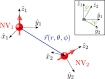
\includegraphics[width=.7\textwidth]{Figures/Shema_annexe}
\caption{Schematics of the ``normal" NV center NV$_s$ and the fluctuator NV$_f$ in and their respective basis ($\hat x_s,\hat y_s,\hat z_s$) and ($\hat x_f,\hat y_f,\hat z_f$), as well as the relative position $\mathbf{r}(r,\theta,\phi)$ between the two spins.}
\label{shema spins annexe}
\end{figure}

The computation of $\bar \eta$ when the single spin Hamiltonian of each spin is diagonal in the magnetic basis $\{ \ket{0}, \ket{+1}, \ket{-1}\}$ was treated in \citep{choi2017depolarization}. We will summarize their results here and consider a few different geometries than the ones presented in the article.

Fig. \ref{shema spins annexe} represents the two spins and the three relevant angles in the problem $\theta,\phi$ and $\psi$. We label with $s$ the properties associated with the ``normal " NV center and $f$ those associated with the fluctuator. For instance the two-qubits state $\ket{m_s=0,m_f=+1}\equiv\ket{0,+1}$ corresponds to the convolution of the single-spin states $\ket{m=0}$ for the NV and $\ket{m=+1}$ for the fluctuator.

The two Cartesian basis ($\hat x_s,\hat y_s,\hat z_s$) and ($\hat x_f,\hat y_f,\hat z_f$) were chosen so that the spin vector Hamiltonian of each spin could be written:
\begin{equation}
\mathbf{S}_i=S_x \hat x_i + S_y \hat{y}_i + S_z \hat{z}_i,
\end{equation}
where :
\begin{align*}
S_x&=\begin{pmatrix}
0&1/\sqrt{2}&0 \\
1/\sqrt{2}&0&1/\sqrt{2} \\
0&1/\sqrt{2}&0
\end{pmatrix} \\
S_y&=\begin{pmatrix}
0&i/\sqrt{2}&0 \\
-i/\sqrt{2}&0&i/\sqrt{2} \\
0&-i/\sqrt{2}&0
\end{pmatrix} \\
S_z&=\begin{pmatrix}
-1&0&0 \\
0&0&0 \\
0&0&+1
\end{pmatrix}.
\end{align*}

The relative position between the two spins is noted with the vector $\mathbf{r}=r\hat{u}$. The vector's spherical coordinate are given in the Cartesian basis of the NV center ($\hat x_s,\hat y_s,\hat z_s$).

The angle $\psi$ between the two spins $z$ axes is defined by the crystal lattice and can take three values within [0,$\pi$] which are: 0 (same class), $\cos^{-1}(1/3) \approx 70.5\ ^\circ$ and $\cos^{-1}(-1/3) \approx 109.5\ ^\circ$. Two distinct classes can either have a relative angle $\psi=70.5 \ ^\circ$ or $\psi=109.5 \ ^\circ$ depending on the external magnetic field: we choose by definition that $\mathbf{B}\cdot\hat{z}_i >0$, which imposes the orientation of $z_i$ and therefore the angle between $\hat z_s$ and $\hat z_f$. This point will be further developed when discussing the $\{100\}$ and $\{110\}$ type resonances.

The direction $\hat x_s=\hat x_f$ is chosen arbitrarily to be : $$\hat x=\frac{\hat z_s \times \hat z_f}{\norm{\hat z_s \times \hat z_f}}.$$
The arbitrary choice of the $\hat x$ direction is justified by the symmetry of the problem in the ($\hat x, \hat y$) plane. We chose here to neglect the symmetry-breaking part of the transverse magnetic field which is justified by the fact that we do not take into consideration the mixing of the eigenstates caused by the transverse field.

Following the notation introduced in \citep{choi2017depolarization}, we can rewrite the dipole-dipole Hamiltonian as:
\begin{equation}
\mathcal{H}_{\rm dd} \approx -\frac{J_0}{r^3}\left[(g+ih)(\ket{0,+1}\bra{+1,0}+\ket{0,-1}\bra{-1,0}) + h.c. + q S_z^sS_z^f \right],
\end{equation}
with 
\begin{align}
g&=\frac{1}{2}\left[3(\hat{u}\cdot\hat{x}_s)(\hat{u}\cdot\hat{x}_f) - (\hat{x}_s \cdot \hat{x}_f) + 3(\hat{u}\cdot\hat{y}_s)(\hat{u}\cdot\hat{y}_f) - (\hat{y}_s \cdot \hat{y}_f) \right] \\
h&=\frac{1}{2}\left[3(\hat{u}\cdot\hat{x}_s)(\hat{u}\cdot\hat{y}_f) - (\hat{x}_s \cdot \hat{y}_f) - 3(\hat{u}\cdot\hat{y}_s)(\hat{u}\cdot\hat{x}_f) + (\hat{y}_s \cdot \hat{x}_f) \right] \\
q&= 3(\hat{u}\cdot \hat{z}_s)(\hat{u}\cdot \hat{z}_f) - (\hat{z}_s \cdot \hat{z}_f).
\end{align}

We should note that the double flips have been omitted because we consider here the case $B\neq0$ for which the $\ket{+1}$ and $\ket{-1}$ states of each spin are far out of resonance.

Eq. \ref{eq. eta debut annexe} can then be written:
\begin{equation}
\eta^2=\frac{1}{3} (\abs{g}^2 + \abs{h}^2) \frac{4\gamma_f^2}{(\omega_f - \omega_{NV})^2+4\gamma_f^2}.
\end{equation}

In order to compute $\bar \eta$, we first decompose $\eta$ as a product of $R$ and $G$ as defined in [REF]:
\begin{equation}
\eta^2=G^2(\theta, \phi, \psi) R^2(\omega_f,\omega_{NV})
\end{equation}
with
\begin{align*}
G^2(\theta, \phi, \psi)&=\frac{1}{3}\left(\abs{g}^2+\abs{h}^2 \right),  \\ 
R^2(\omega_f,\omega_{NV}) &= \frac{4\gamma_f^2}{(\omega_f - \omega_{NV})^2+4\gamma_f^2}.
\end{align*}

$R$ and $G$ can be averaged separately as they do not depend on the same variables, which means that:
\begin{equation}
\label{eq. eta bar r bar g bar}
\bar \eta = \bar R \cdot \bar G.
\end{equation} 

The computation of $\bar{R}$ has been discussed in [REF], we will focus here on $\bar{G}$ defined as:

\begin{equation}
\label{eq. eta base mag}
\bar{G}= \iint \abs{G} \frac{\rm d\theta \cos \theta \rm d\phi}{4 \pi}.
\end{equation}

Eq. \ref{eq. eta base mag} can be solved analytically for the case $\psi=0$ and numerically for $\psi=70.5 \ ^\circ$ or $\psi=109.5 \ ^\circ$. The three values are reported in Table \ref{table G mag}. The values found for $\psi=0$ and $\psi=70.5 \ ^\circ$ are the same that were found by the authors of \citep{choi2017depolarization} \footnote{They differ by a factor $\sqrt{1/3}$ because of the definition of $G$.}.

\begin{table}[htbp]
\centering
\caption{Computation of $\bar G$ in the magnetic basis}
 \label{table G mag}
\begin{tabular}{c|c|c}
\toprule
$\psi=0$ & $\psi=70.5 \ ^\circ$ & $\psi=109.5 \ ^\circ$ \\

$\frac{2}{9}=0.222$ & 0.3757 & 0.4808 \\
\bottomrule
\end{tabular}
\end{table}

\subsection{Interclass resonance and magnetic field orientation}

\begin{figure}[h]
\centering
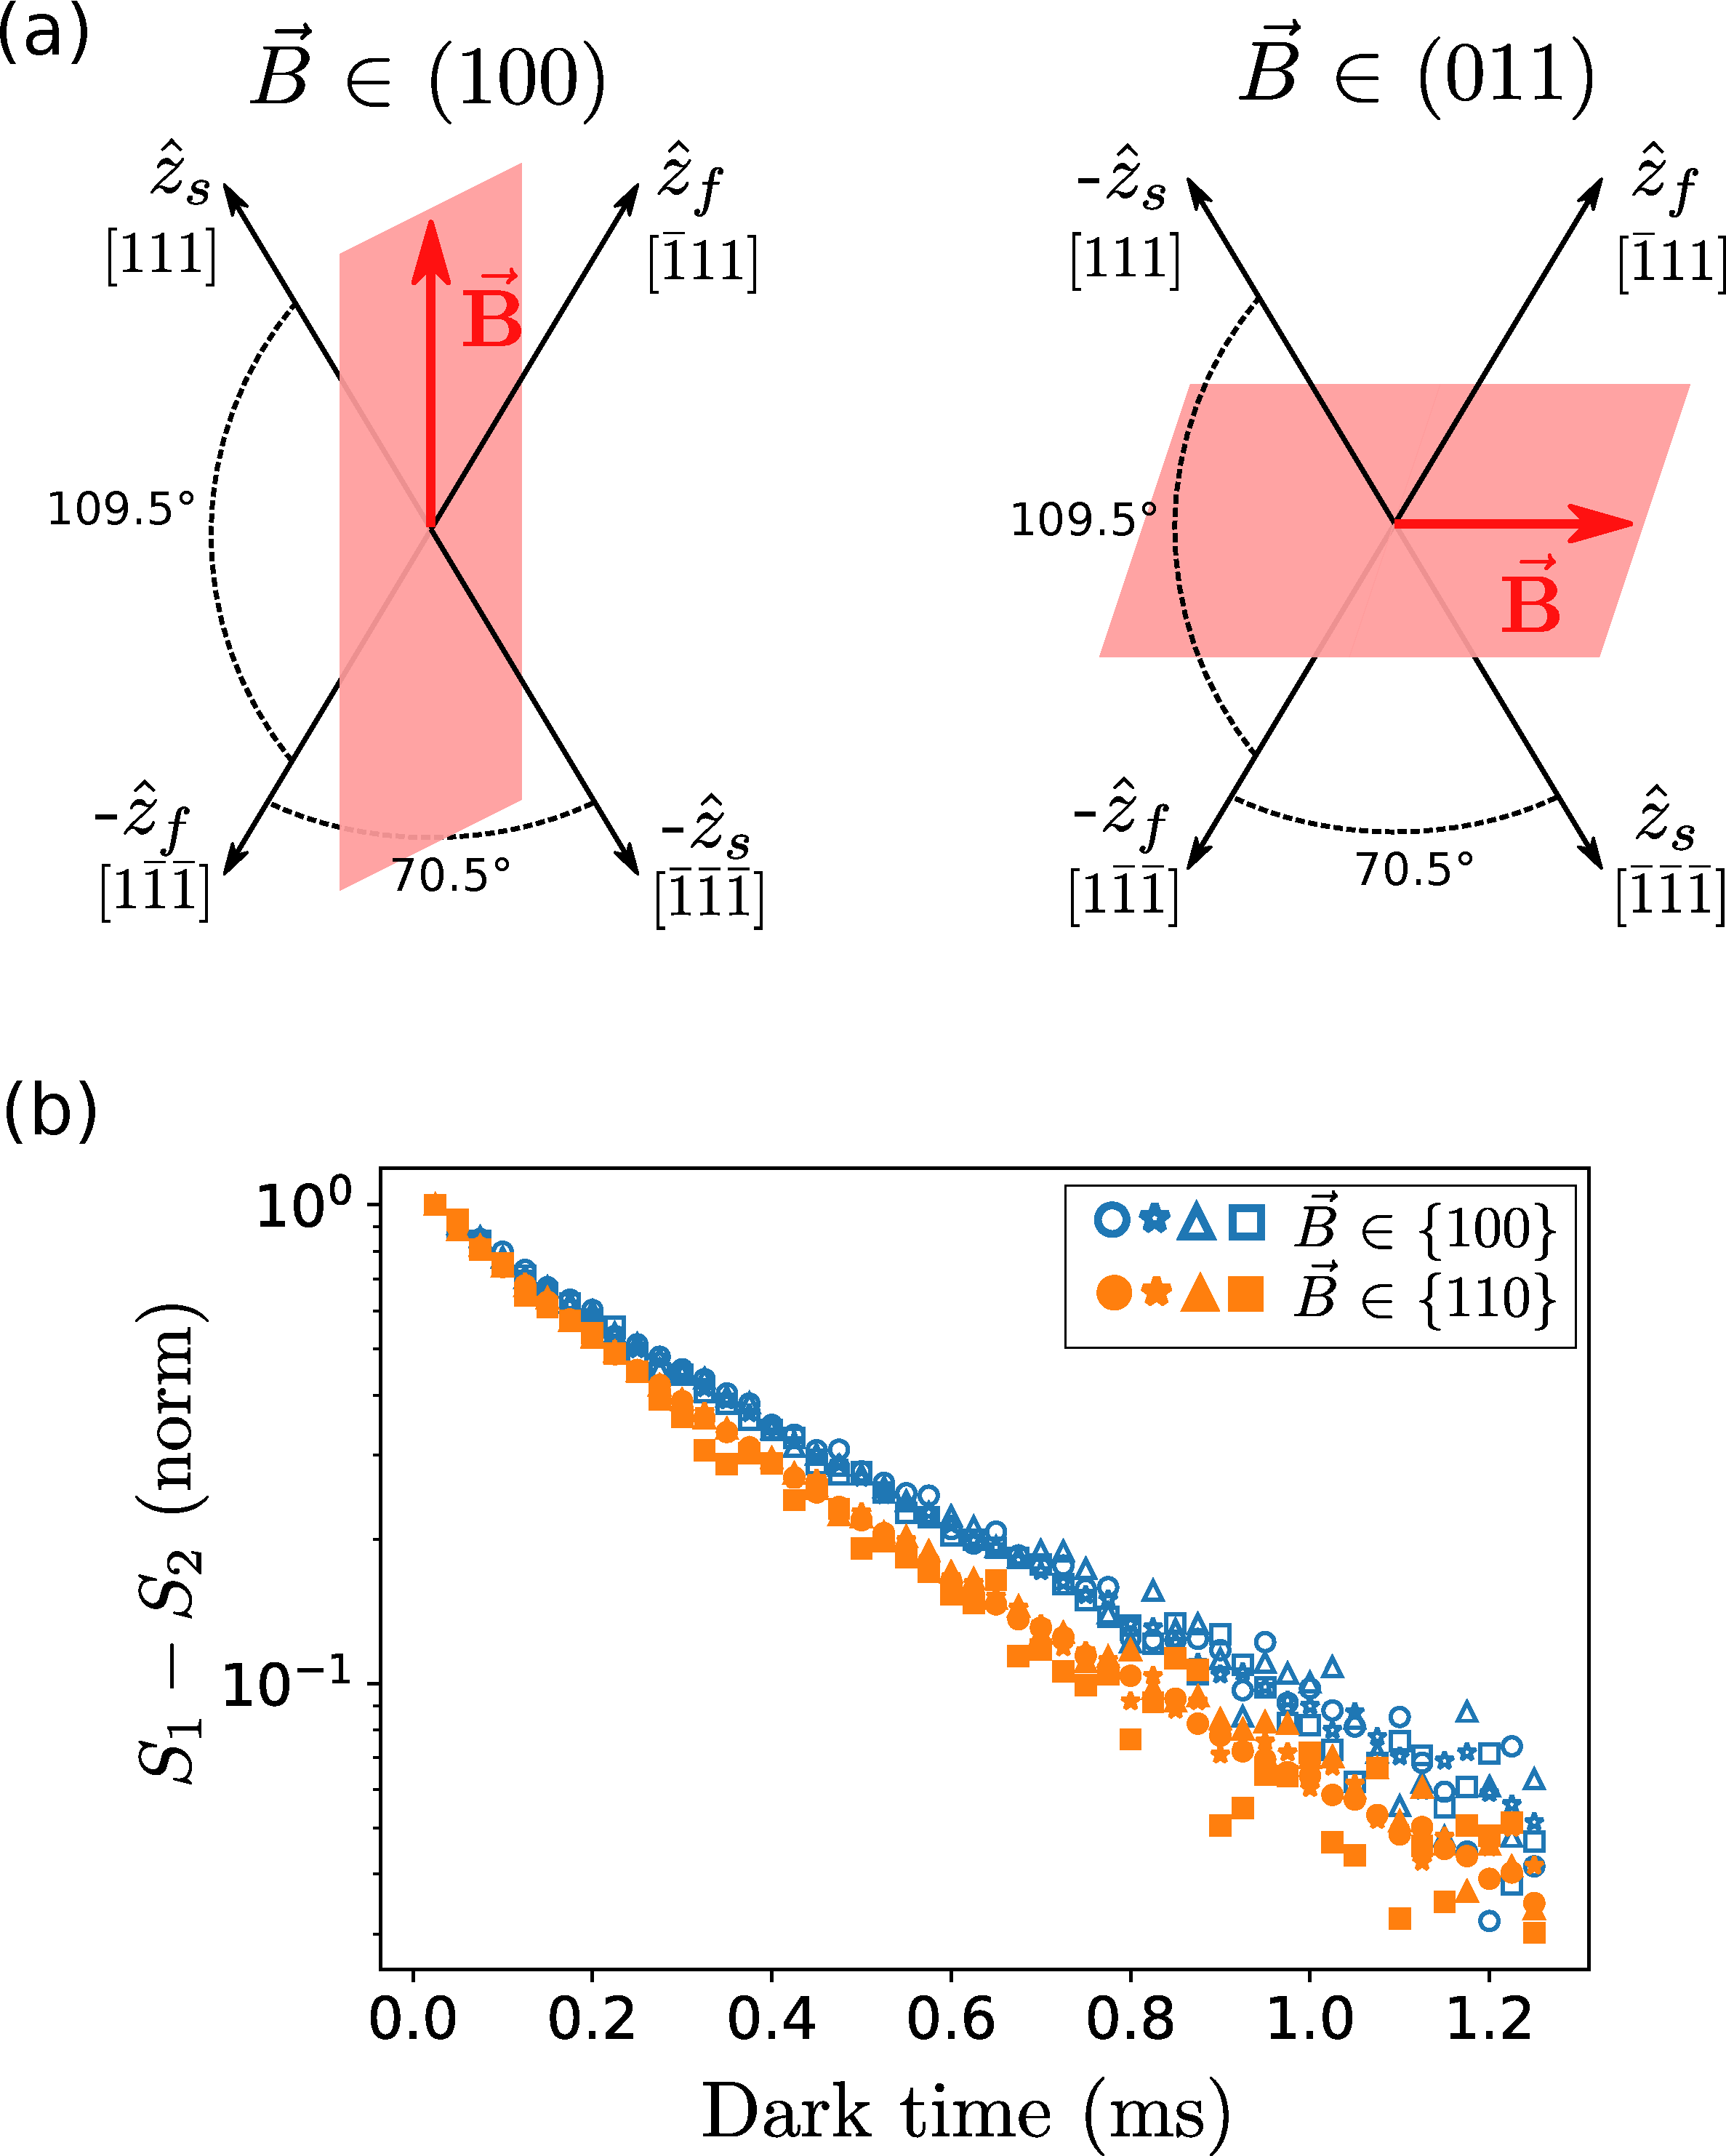
\includegraphics[width=.8\textwidth]{Figures/110_vs_100}
\caption{(a) Illustration of the co-resonance condition between a NV center parallel to the [111] axis and a fluctuator parallel to the [$\bar 1$11] axis. The $\hat z$ direction is defined by the condition $\mathbf{B}\cdot\hat{z} >0$. (b) 8 individual $T_1$ measurements on sample ADM-15-3 on a two-class resonance for 8 different values of the magnetic field (4 $\mathbf{B} \in \{110\}$ and 4 $\mathbf{B} \in \{100\}$).}
\label{110 vs 100 annexe}
\end{figure}

As discussed in sec [REF], there are 4 possibles magnetic field orientations for which at least two NV classes are co-resonant: $\mathbf{B} \in \{110\}$ (two-class resonance), $\mathbf{B} \in \{100\}$ (2$\times$two-class resonance), $\mathbf{B} \parallel \langle 111 \rangle$ (three-class resonance) and $\mathbf{B} \parallel \langle 100\rangle$ (four-class resonance).

Fig. \ref{110 vs 100 annexe}-a) illustrates the difference in the angle $\psi$ for the case $\mathbf{B} \in \{110\}$ and $\mathbf{B} \in \{100\}$. We consider here an NV center parallel to the [111] axis and a fluctuator parallel to the [$\bar 1$11] axis. Without external fields, the $\hat z$ direction of the NV center could be either [111] or [$\bar 1 \bar 1 \bar 1$], however the condition $\mathbf{B}\cdot\hat{z} >0$ imposes in the left case $\hat z_s=[111]$ and in the right cases $\hat z_f=[\bar 1 \bar 1 \bar 1]$. 

For the NV center and the fluctuator to be resonant, the magnetic field needs to have the same projection on the $\hat z_s$ and $\hat z_f$ axes, which in this case means either $\mathbf{B} \in (100)$ or $\mathbf{B} \in (011)$. The angle $\psi$ between the $\hat z_s$ and $\hat z_f$ axes however is different in both cases. The same can be generalized for every $\mathbf{B} \in \{110\}$ and $\mathbf{B} \in \{100\}$ type resonance: the angle $\psi \in [0,\pi]$ between two resonant classes is equal to $70.5 \ ^\circ$ for a $\mathbf{B} \in \{100\}$ type resonance, and $109.5 \ ^\circ$ for a $\mathbf{B} \in \{110\}$ type resonance.

Because $\bar G$ is greater for $\psi=109.5 \ ^\circ$ than it is for $\psi=70.5 \ ^\circ$, then following eq. \ref{eq. eta bar r bar g bar}, we should expect a faster depolarization rate when $\mathbf{B} \in \{110\}$ than when $\mathbf{B} \in \{100\}$. Fig. \ref{110 vs 100 annexe}-b) Shows 8 different $T_1$ measurement performed on the same sample for 8 different magnetic fields, four of which were in the $\mathbf{B} \in \{110\}$ scenario and four in the $\mathbf{B} \in \{100\}$ scenario. We can clearly see a slower relaxation rate for all four $\mathbf{B} \in \{100\}$ measurements compared to all four $\mathbf{B} \in \{110\}$, which agrees with the predictions of the model.

For a perfect resonance matching (i.e. no detuning between the central frequencies of the different resonant classes), we can assume that $\bar R$ is a constant ($\bar R \equiv \bar R^0 \approx \frac{2 \gamma_f}{2 \gamma_f + \Gamma_f + \Gamma_{NV}}$ according to eq. [REF]). We then have:

\begin{align}
\bar \eta(\rm{1\ class})&=\bar G(\psi=0) \bar R_0 \\[1em]
\frac{\bar \eta(\mathbf{B} \in \{110\})}{\bar \eta(\rm{1\ class})}&= \frac{\bar G(\psi=70.5 \ ^\circ)+ \bar G(\psi=0)}{\bar G(\psi=0)}\\[1em]
\frac{\bar \eta(\mathbf{B} \in \{100\})}{\bar \eta(\rm{1\ class})}&= \frac{\bar G(\psi=109.5 \ ^\circ)+ \bar G(\psi=0)}{\bar G(\psi=0)}\\[1em]
\frac{\bar \eta(\mathbf{B} \parallel \langle 111 \rangle)}{\bar \eta(\rm{1\ class})}&= \frac{2\bar G(\psi=109.5 \ ^\circ)+ \bar G(\psi=0)}{\bar G(\psi=0)}\\[1em]
\frac{\bar \eta(\mathbf{B} \parallel \langle 100 \rangle)}{\bar \eta(\rm{1\ class})}&= \frac{2\bar G(\psi=70.5 \ ^\circ)+ \bar G(\psi=109.5 \ ^\circ) + \bar G(\psi=0)}{\bar G(\psi=0)}
\end{align} 

Finally, the values in Table [REF] are computed thanks to the relation: \begin{equation}
\frac{\Gamma_1}{\Gamma_0}= \left(\frac{\bar \eta}{\bar \eta(\rm{1\ class})} \right)^2.
\end{equation}

Note that we only give here the relaxation rates for a single class. To estimate the total PL, one would need to compute the relaxation rate of all 4 classes independently, for instance in a $\mathbf{B} \in \{110\}$ scenario, two classes have a relaxation rate $\Gamma(\mathbf{B} \in \{110\})$ and two classes have a relaxation rate $\Gamma_0$.
\printbibliography
\end{document}